% !TEX root=ricardo_draft.tex
%%% TeX-master: "ricardo_draft"~\ref{figure.simple_models}

% \begin{center}
  % \begin{tabular}{c}
  %   Here, a graph $U_A \rightarrow A \rightarrow Y \leftarrow U_Y$
  %   (rearrange it spatially in any way you want (including this table).)\\ (a)\\ \\
  %   Here, a graph made of edges \\
  %   $A \leftarrow U_A$, $Employed \leftarrow \{A, Prejudiced, Qualifications\}$,
  %   $Y \leftarrow \{Employed, U_Y\}$. \\ (b)\\ \\
  %   Here, a twin network,
  %   $A \leftarrow U_A$, $Employed \leftarrow \{A, Prejudiced, Qualifications\}$,
  %   $Y \leftarrow \{Employed, U_Y\}$,\\
  %   $Employed_a \leftarrow \{a, Prejudiced, Qualifications\}$,
  %   $Y_a \leftarrow \{Employed_a, U_Y\}$,\\
  %   $Employed_{a'} \leftarrow \{a', Prejudiced, Qualifications\}$,
  %   $Y_{a'} \leftarrow \{Employed_{a'}, U_Y\}$,
  %   (``$a$'' and ``$a'$'' are two extra nodes too)\\.
  %   \\ (c)\\
  % \end{tabular}
  % \label{fig:ex1}
  % \caption{(a) The graph corresponding to a causal model with $A$ being the protected outcome
  %   and $Y$ some outcome of interest, with background variables assumed to be independent.
  %   (b) Expanding the model to include an intermediate variable indicating whether the individual
  %   is employed with two (latent) background variables $\textbf{Prejudiced}$ (whether the person in charge
  %   of offering the job is prejudiced) and $\textbf{Qualifications}$ (a measure of the qualifications of
  %   the individual). (c) A twin network representation of this system \citep{pearl:00}
  %   under two different counterfactual levels for $A$. The network is created by creating copies
  %   of nodes descending from $A$, which inherit parents from the factual world that have not
  %   been affected.}
% \end{center}
%\end{figure}


%\subsection{Definition}
%Formally, a variable $Y$ is said to be counterfactually fair with
%respect to a protected attribute $A$ if
Given a predictive problem with fairness considerations, where $A$, $X$ and $Y$
represent the protected attributes, remaining attributes, and output of interest respectively,
let us assume that we are given a causal model $(U, V, F)$, where $V \equiv A \cup X$.
We postulate the following criterion for predictors of $Y$.
\begin{define}[Counterfactual fairness]
Predictor $\hat Y$ is {\bf counterfactually fair}
if under any context $X = x$ and $A = a$,
  \label{eq:cf_definition}
\begin{align}
  P(\hat Y_{A \leftarrow a\ }(U) = y\ |\ X = x, A = a)  =%\nonumber\\ 
  P(\hat Y_{A \leftarrow a'}(U) = y\ |\ X = x, A = a), 
\end{align}
for all $y$ and for any value $a'$ attainable by $A$.
\end{define}
%Simply put,

This is closely related to
{\bf actual causes} \cite{halpern:16}, or token causality in the sense
that, to be fair, $A$ should not be a cause of $\hat Y$ in any
individual instance. In other words, changing $A$ while holding things
which are not causally dependent on $A$ constant
will not change the distribution of $\hat Y$.
% \footnote{Notice that we always assume counterfactuals to be
%  well-defined by the model. For instance, ``race'' can be taken as a
%  surrogate for ``perceived race.''}
We also emphasize that
counterfactual fairness is an individual-level definition. This is
substantially different from comparing different individuals that happen to
share the same ``treatment'' $A = a$ and coincide on the values of
$X$, as discussed in Section 4.3.1 of \citep{pearl:16} and the
Supplementary Material\footnote{We strongly suggest that reviewers
  look at it.}. Differences between $X_a$ and $X_{a'}$ must be caused
by variations on $A$ only. Notice also that this definition is
agnostic with respect to how good a predictor $\hat Y$ is, which we
discuss in Section \ref{sec:methods}.

\noindent {\bf Relation to individual fairness}. IF is agnostic with
respect to its notion of similarity metric, which is both a strength
(generality) and a weakness (no unified way of defining similarity).
Counterfactuals and similarities are related, as in the classical
notion of distances between ``worlds'' corresponding to different
counterfactuals \cite{lewis:73}. Defining $\hat Y$ as a
deterministic function of $W \subset A \cup X \cup U$, as in several
of our examples to follow, then IF can be defined by treating equally two
individuals with the same $W$ in a way that is also counterfactually fair.

\noindent {\bf Relation to \citet{pearl:16}}.  In
Example 4.4.4 of \cite{pearl:16}, the authors condition instead on
$X$, $A$, and the observed realization of $\hat Y$, and calculate the
probability of the counterfactual realization $\hat Y_{A \leftarrow
  a'}$ differing from the factual.
%\footnote{The result is an expression
%  called the ``the probability of sufficiency'' for $A$, capturing the
%  notion that switching $A$ to a different value would be sufficient
%  to change $\hat Y$ with some probability.}.
This example conflates the predictor $\hat Y$ with the outcome $Y$, of
which we remain agnostic in our definition but which is used in the
construction of $\hat Y$ as in Section \ref{sec:methods}. Our framing
makes the connection to machine learning more explicit.
% We also emphasize that counterfactual fairness is an individual-level
% definition. This is substantially different from the notion of ``causal independence''
% as discussed in Section 4.3.1 of \cite{pearl:16}. Causal independence
% % requires
% % \begin{align}
% %   &P(\hat Y = y\ |\ do(A = a), W = w) =\nonumber\\ 
% %   &P(\hat Y = y\ |\ do(A = a'), W = w),
% % \end{align}
% % which
% entails comparing different units that happen to share the
% same ``treatment'' and coincide on values of $W$, while
% counterfactual fairness concerns the variation possible within an
% individual depending on their value of $a$ and the descendents of
% $A$ in the causal graph.

\begin{figure}
  \begin{tabular}{p{0.5\columnwidth}|p{0.5\columnwidth}}
    \centerline{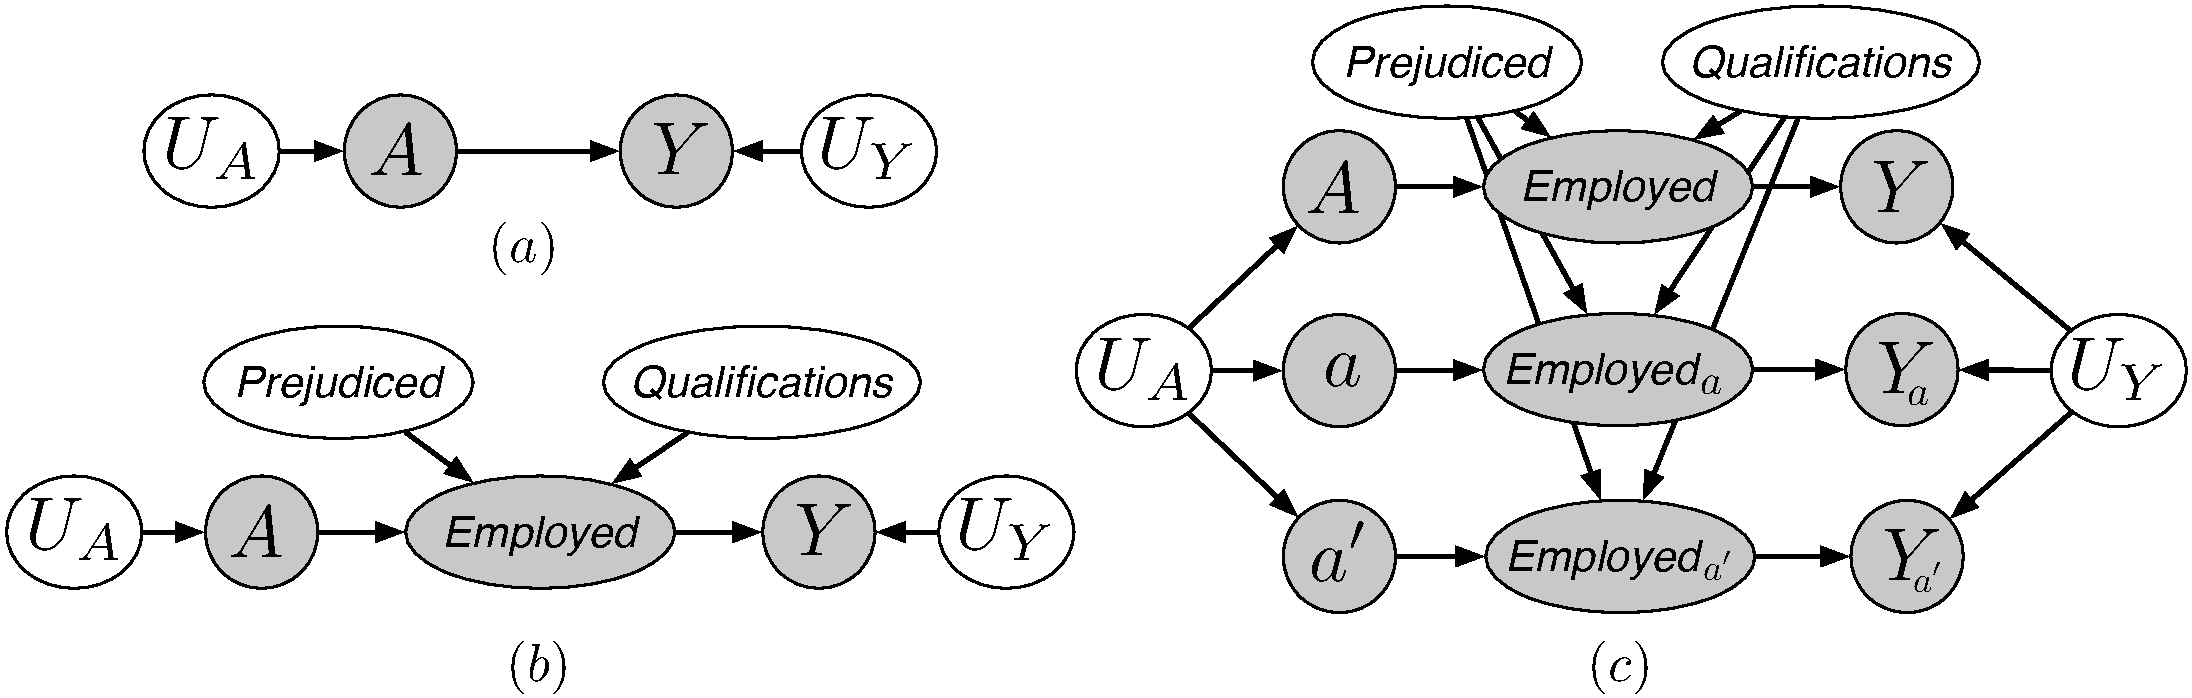
\includegraphics[width=0.5\columnwidth]{implications_fig.pdf}}&
    \centerline{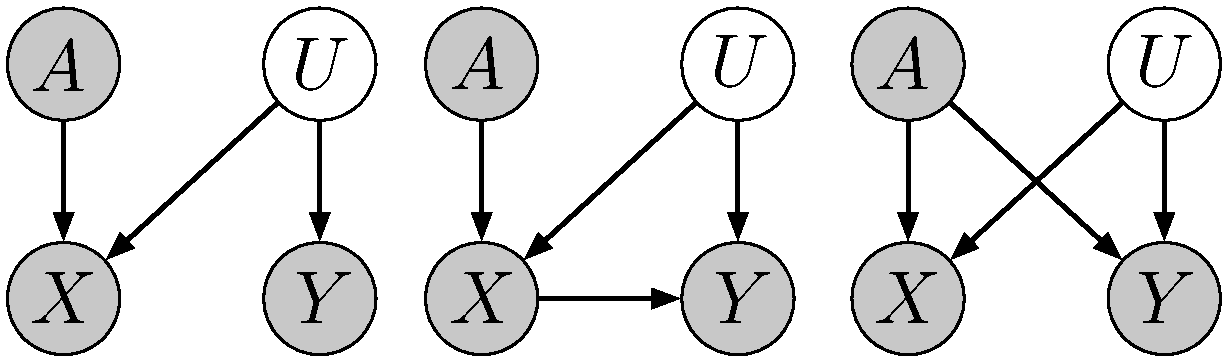
\includegraphics[width=0.5\columnwidth]{simple_models_no_q3}}(d)
  \end{tabular}
  \caption{\label{fig:ex1} {\bf Left:} (a) The graph corresponding to
    a causal model with $A$ being the protected attribute and $Y$ some
    outcome of interest, with background variables assumed to be
    independent.  (b) Expanding the model to include an intermediate
    variable indicating whether the individual is employed with two
    (latent) background variables $\textbf{Prejudiced}$ (if the person
    offering the job is prejudiced) and $\textbf{Qualifications}$ (a
    measure of the individual's qualifications). (c) A twin network
    representation of this system \citep{pearl:00} under two different
    counterfactual levels for $A$. This is created by copying nodes
    descending from $A$, which inherit unaffected parents from the
    factual world. (d) Two causal models for different
    real-world fair prediction scenarios.\label{figure.simple_models}
    See Section \ref{sec:count_fair} for discussion.}
\end{figure}

\subsection{Implications}
%
One simple but important implication of the definition of counterfactual fairness is the following:
%
\begin{lem}
  \label{lem:nondescend}
  Let $\mathcal G$ be the causal graph of the given model $(U, V, F)$.
  Then $\hat Y$ will be counterfactual fair if it is a function
  of the non-descendants of $A$.
\end{lem}
%
\begin{proof}
 Let $W$ be any non-descendant of $A$ in $\mathcal G$. Then $W_{A
   \leftarrow a}(U)$ and $W_{A \leftarrow a'}(U)$ have the same
 distribution by the three inferential steps in Section
 \ref{subsec:cmc}.  Hence, the distribution of any function $\hat Y$ of the non-descendants of $A$
 is invariant with respect to the counterfactual values of $A$.
\end{proof}

This does not exclude using a descendant $W$ of $A$ as a possible input to
$\hat Y$. However, this will only be possible in the case where the
overall dependence of $\hat Y$ on $A$ disappears, which will not
happen in general. Hence, Lemma~\ref{lem:nondescend} provides the most
straightforward way to achieve counterfactual fairness.

\noindent{\bf Ancestral closure of protected attributes.} Suppose that
a parent of a member of $A$ is not in $A$.  Counterfactual fairness
allows for the use of it in the definition of $\hat Y$. If this seems
counterintuitive, then we argue that the fault should be at the
postulated set of protected attributes rather than with the definition
of counterfactual fairness, and that typically we should expect set
$A$ to be closed under ancestral relationships given by the causal
graph. For instance, if {\it Race} is a protected attribute, and {\it
  Mother's race} is a parent of {\it Race}, then it should also be in
$A$.

\noindent{\bf Dealing with historical biases.} The explicit difference
between $\hat Y$ and $Y$ allows us to tackle historical biases. For
instance, let $Y$ be an indicator of whether a client defaults on a
loan, while $\hat Y$ is the actual decision of giving the
loan. Consider the DAG $A \rightarrow Y$, shown in Figure
\ref{fig:ex1}(a) with the explicit inclusion of set $U$ of independent
background variables. $Y$ is the objectively ideal measure for
decision making, the binary indicator of the event that the individual defaults on
a loan. If $A$ is postulated to be a protected attribute, then the
predictor $\hat Y = Y = f_Y(A, U)$ is not counterfactually fair, with the arrow $A
\rightarrow Y$ being (for instance) the result of a world that
punishes individuals in a way that is out of their control. Figure
\ref{fig:ex1}(b) shows a finer-grained model, where the path is
mediated by a measure of whether the person is employed, which is
itself caused by two background factors: one representing whether the
person hiring is prejudiced, and the other the employee's
qualifications. In this world, $A$ is a cause of defaulting, even if
mediated by other variables\footnote{For example, if the function
  determining employment $f_E(A,P,Q) \equiv I_{(Q > 0, P = 0 \text{ or } A
    \neq a)}$ then an individual with sufficient qualifications and
  prejudiced potential employer may have a different counterfactual
  employment value for $A = a$ compared to $A = a'$, and a different
  chance of default. }. The counterfactual fairness principle however
forbids us from using $Y$: using the twin network of \citet{pearl:00},
we see in Figure \ref{fig:ex1}(c) that $Y_a$ and $Y_{a'}$ need not be
identically distributed given the background variables.
  % \footnote{We assume
  % that function $f_Y(A, U)$ is not pathological, that is, it will give
  % different outcomes for different values of $A$ other things being
  % equal. Moreover, we assume interventions in $A$ are well defined.
  % For instance, ``race'' here could be formulated as ``race
  % perception'', which can be due to, for instance, to
% racially-associated names in a C.V. or loan application.}

In contrast, any function of variables not descendants of $A$ can be
used a basis for fair decision making. This means that any variable
$\hat Y$ defined by $\hat Y = g(U)$ will be counterfactually fair for
any function $g(\cdot)$. Hence, given a causal model, the functional
defined by the function $g(\cdot)$ minimizing some predictive error
for $Y$ will satisfy the criterion, as proposed in Section
\ref{sec:algorithm}. We are essentially learning a projection of $Y$
into the space of fair decisions, removing historical biases as a
by-product.

% There are two issues to be clarified at this point. First,
% it sounds potentially counter-intuitive that our definition
% seemingly allows for the use of (background) variable $\textbf{Prejudiced}$
% directly. However, our point of view is that there is no harm: this is
% a feature of some other person who judged a job application of the
% individual concerned, not a feature of the individual. This variable
% might prove itself to be a useless predictor of $Y$ depending on the
% structural equations, resulting from the marginalization of $A$, but
% in principle it is not harmful as implied by the model.

% The second and more complicated issue concerns the fact that
% However, it appears to be the case that $\hat Y$ and $A$ will be
% ``causally dependent'' in general given $W$, meaning that $P(\hat Y =
% y\ |\ do(A = a), W = w) \neq P(\hat Y = y\ |\ do(A = a'), W = w)$.
% Our argument on why this is not a problem mirrors the discussion in
% Section 4.3.1 of \cite{pearl:16}, on the differences between
% counterfactual exchangeability and causal independence: the latter is
% a comparison among different units that happen to share the same
% treatment and coincide on the same outcomes for $W$. But in the
% postulated model $W$ responds to $A$ so, starting from a baseline
% individual with treatment $do(A = a)$ and measurements $w$, consider
% the generative model to generate a comparable individual: under $do(A
% = a')$, perform rejection sampling among individuals until we find
% someone who matches our target on the same $w$. This sampling
% mechanism gives a different posterior distribution for $U$ than the
% within-individual distribution\footnote{For example, if $w$ is a
%   common outcome under $do(A = a)$ and $P(U)$, but rare under $do(A =
%   a')$ and $P(U)$.} of the original individual, which is the one we care about in our
% definition. Hence, the inequality
% \begin{align}
%   P(\hat Y = y\ |\ do(A = a), W = w)
%   \neq P(\hat Y = y\ |\ do(A = a'), W = w)
% \end{align}
% should not be a matter of
% concern for a criterion defined for individual level differences.

%%%%%%% ICML STUFF
%Note that we can build counterfactually fair
%predictive models for some $\hat Y$ even if the 
%structural equations that generated $Y$ are unfair. The idea is that we
%are learning a projection of $Y$ into an alternate world where it
%would be fair, which we may think of as a
%``closest world'' defined by our class of models and the
%causal structure of the world\footnote{The notion of ``closest world''
%  is pervasive in the literature of counterfactual inference under
%  different meanings \citep{pearl:00, halpern:16}.  Here, the cost
%  function used to map fair variables to unfair outcomes also plays a
%  role, but this concerns a problem dependent utility function that
%  would be present anyway in the unfair prediction problem, and is
%  orthogonal to the causal assumptions.}.
%%%%%%%% END OF ICML STUFF

\subsection{Further Examples}
\label{sec:further_examples}

To give further intuition for counterfactual fairness, we will consider
two real-world fair prediction scenarios: \textbf{insurance pricing}
and \textbf{crime prediction}. Each of these correspond to one of the
two causal graphs in Figure~\ref{figure.simple_models}(d). The
Supplementary Material provides a more mathematical discussion of
these examples with more detailed insights.

\paragraph{Scenario 1: The Red Car.}
A car insurance company wishes to price insurance for car
owners by predicting their accident rate $Y$. They assume there is an
unobserved factor corresponding to aggressive driving $U$, that (a)
causes drivers to be more likely have an accident, and (b) causes
individuals to prefer red cars (the observed variable $X$). Moreover,
individuals belonging to a certain race $A$ are more likely to drive
red cars. However, these individuals are no more likely to be
aggressive or to get in accidents than any one else. We show this in
Figure~\ref{figure.simple_models}(d) (\emph{Left}). Thus, using the
red car feature $X$ to predict accident rate $Y$ would seem to be an
unfair prediction because it may charge individuals of a certain race
more than others, even though no race is more likely to have an
accident. Counterfactual fairness agrees with this notion, as $X$
is a descendent of $A$ but $U$ is not. Interestingly, we can show
(Supplementary Material) that in a linear model, regression $Y$ on $A$
and $X$ is equivalent to regressing on $U$, so off-the-shelf
regression here is counterfactually fair. Regressing $Y$ on $X$ alone
obeys the FTA criterion but is not counterfactually fair, so
{\em omitting $A$ (FTU) may introduce unfairness into
  an otherwise fair world.}
%
\paragraph{Scenario 2: High Crime Regions.}
%%%%% ICML STUFF
%A local police precinct wants to know $Y$, whether a given house is to
%be broken into in any given day. The probability of $Y = 1$ depends on many
%unobserved factors ($U$) but also upon the neighborhood the house lies
%in ($X$). However, different ethnic groups are more likely to live in
%particular neighborhoods, and so neighborhood and break-in rates are
%often correlated with the race $A$ of the house occupier. This can be
%seen in Figure~\ref{figure.simple_models}(d) (\emph{Center}). Unlike the
%previous case, a predictor $\hat Y$ trained using $X$ and $A$ is not
%counterfactually fair. The only change from Scenario 1 is that now $Y$
%depends on $X$ as follows: $Y \!=\! \gamma U + \theta X$. Now if we
%solve for $\lambda_X,\lambda_A$ it can be shown that $\hat Y(X,a)
%\!=\! (\gamma - \frac{\alpha^2 \theta v_A}{\beta v_U})U + \alpha
%\theta a$. As this predictor depends on the values of $A$, $\hat
%Y(X,a) \!\neq\! \hat Y(X,a')$ and thus $\hat Y(X,A)$ is not
%counterfactually fair.
%%%%% END ICML STUFF
A city government wants to estimate crime rates by neighborhood to
allocate policing resources. Its analyst constructed training data
by merging (1) a registry of residents containing their neighborhood $X$
and race $A$, with (2) police records of arrests, giving each resident a
binary label with $Y = 1$ indicating a criminal arrest record.
Due to historically segregated housing, the location $X$ 
depends on $A$.
Locations $X$ with more police resources have larger numbers of
arrests $Y$.
And finally, $U$ represents the totality of socioeconomic factors
and policing practices that both influence where an individual may
live and how likely they are to be arrested and charged.
This can all be seen in Figure~\ref{figure.simple_models}(d)
(\emph{Right}).

In this example,
higher observed arrest rates in some neighborhoods
are due to greater policing there, not because people of different races
are any more or less likely to break the law.
The label $Y = 0$ does not
mean someone has never committed a crime, but rather that they have not
been caught.
{\em If individuals in the training data have not already had equal
  opportunity, algorithms enforcing EO will not remedy such unfairness}.
In contrast, a counterfactually fair approach would model
differential enforcement rates using $U$ and base predictions
on this information rather than on $Y$ directly.

% Unlike Scenario 1, $Y$ now
% depends on $X$ directly. If all structural equations are linear, then
% $U$ is a linear function of $A$ and $X$, and so, indirectly, a
% counterfactually fair $\hat Y$ can be expressed as a linear function
% of $A$ and $X$. However, this is different from assuming that $\hat Y$ can be
% \emph{any} linear combination of $A$ and $X$. As a matter of fact, the solution for the
% unrestricted least-squares regression of $Y$ on $A$ and $X$ cannot be
% written as a function of $U$ only, as shown in the Supplementary Material.
%Intuitively this is because the predictor $\hat Y(X,A)$ will be a
% function of not only $U$, but also of the part of $X$ that directly
% causes $Y$. This means that the change in $X$ caused by the
% counterfactual change in $A$ from $a$ to $a'$ will cause a change in
% $\hat Y(X,A)$ so that $\hat Y(X,a) \!\neq\! \hat Y(X,a')$.  In such
% a scenario, although the likelihood of a particular person having
% their house broken into does not depend upon race directly, it does
% vary which a persons race and so is not counterfactually fair.

In general, we need a
multistage procedure in which we first derive latent variables $U$, and
then based on them we minimize some loss with respect to $Y$. This is the
core of the algorithm discussed next.

%%%%%%%% ICML STUFF
%\paragraph{Scenario 3: University Success.}
%A university wants to know if students will be successful
%post-graduation $Y$. They have information such as: grade point
%average (GPA), advanced placement (AP) exams results, and other
%academic features $X$. The university believes however, that an
%individual's gender $A$ may influence these features and their
%post-graduation success $Y$ due to social discrimination. They also
%believe that independently, an individual's latent talent $U$ causes
%$X$ and $Y$. We show this in Figure~\ref{figure.simple_models}(d)
%(\emph{Right}). We can again ask, is the predictor $\hat Y(X,A)$
%counterfactually fair? In this case, the different between this and
%Scenario 1 is that $Y$ is a function of $U$ and $A$ as follows: $Y
%\!=\! \gamma U + \eta A$. We can again solve for $\lambda_X,\lambda_A$
%and show that $\hat Y(X,a) \!=\! (\gamma - \frac{\alpha \eta
%  v_A}{\beta v_U})U + \eta a$. Again $\hat Y(X,A)$ is a function of
%$A$ so it cannot be counterfactually fair.
%%%%%%%% END ICML STUFF

% TODO. Here the main
% definition is introduced, and how it relates to ``path deletion'',
% including the core example of $A \rightarrow X \rightarrow Y$, with
% two latent variables $U_x \rightarrow X$ and $U_y \rightarrow Y$,
% arguing that one might judge that the path from $A$ to $Y$ via is due
% to an unfair mechanism and that we need a notion of ``closest world''.


% When describing counterfactual fairness, it is important to
% distinguish between a counterfactually fair {\em world} in which the
% variable $Y$ we are interested in predicting is inherently
% counterfactually fair with respect to the protected attributes $A$,
% and a counterfactually fair {\em predictor} $\hat Y$, guaranteed to
% be counterfactually fair, regardless of the behavior of $Y$.

% Figure~\ref{figure.simple_models} shows possible worlds. {\em Left:} A
% counterfactually fair world in which the state of $Y$ has no
% dependencies on $A$. {\em Center and Right:} Potentially unfair worlds
% in which the state of $A$ can influence the state of $Y$ either
% indirectly as in {\em center} or directly as in {\em Right}.

%In Scenarios 2 and 3 in general $\hat Y(X,A)$ will also not satisfy demographic parity as $Y$ will be affected by $A$. In fact, we demonstrate in the next section that demographic parity is strictly more restrictive than counterfactual fairness.

%  The world on the right shows $Y'$ a
% causally fair variable that doesn't depend on $A$ being directly
% corrupted by a bias relating to $A$, resulting in an observation
% $Y$. In this case, learning a causally fair approximation of $Y$ can
% recover the true variable $Y'$ (up to noise).


% \subsection{Examples}
% To get an intuition for what the different definitions of fairness imply, we will
% revisit the examples of figure \ref{figure.simple_models}.
% begin by describing a few possible real-world scenarios. For each of these we will describe what counterfactually-fair and counterfactually-unfair predictors look like.

% \paragraph{Scenario 1: The Red Car.}
% Imagine a car insurance company wants a quick, anonymous way to determine how to price insurance for different car owners by predicting their accident likelihood $Y$. They've noticed that there is a correlation between driving a red car $X$ and a higher rate of automobile accidents. Thus they would like to increase the insurance for all red car drivers. 

% Imagine what's really going on is shown in Figure~\ref{figure.simple_models} (\emph{Left}). The correlation between have a red car $X$ and accidents $Y$ is due to an `aggressiveness' factor $U$: aggressiveness causes individuals to be in accidents more often, and it also attracts them to red cars. Unfortunately, the red car feature $X$ is also affected by an individual's race $A$. 

% TODO. Here the examples and their motivation can be as follows:

% \begin{itemize}
% \item something analogous to the red car example: $A$ is not a cause of
%   $Y$ but might indirectly bias the result even without using $A$ as a predictor;
% \item something with selection bias, maybe a toy version of COMPAS;
% \item something where an unfair judgment (say, credit score) that can be potentially
%   considered as a target variable, and an
%   ``objective target'' (say, defaulting on a loan) are present, and
%   what the recommendation is
% \end{itemize}
%%% Local Variables:
%%% mode: latex
%%% TeX-master: "ricardo_draft"
%%% End:
